\subsection{Cover lattice example}

Converting the program in \autoref{lst:lattices-program} to a program graph, one gets the program graph displayed in \autoref{fig:termination-example-graph}.

\begin{listing}
    \begin{minted}{bash}
        i := 0;
        while true do i := i + 1
    \end{minted}
    \caption{A program where cover lattices are required for termination}
    \label{lst:lattices-program}
\end{listing}

\begin{figure}
    \centering
    \begin{tikzpicture}
    \tikzstyle{arrow} = [thick,->,>=stealth]
    \node [circle, draw] (start) at (0,0){$q_{\whitepointerright}$};
    \node [circle, draw] (a) at (0,-1.5) {$q_1$};
    \node [circle, draw] (b) at (0,-4) {$q_2$};
    \node [circle, draw] (end) at (0,-5.5) {$q_\blackpointerleft$};


    \draw[arrow, ->] (start) to node[right] {$i:=0$} (a);
    \draw[arrow, ->] (a) to node[left, xshift=2] {$true$} (b);

    \draw[arrow, ->] (b) edge[bend right=50] node[right]{$i:=i+1$} (a);

    \draw[arrow, ->] (a) edge[bend right=70] node[left]{$\neg true$} (end);
\end{tikzpicture}
    \caption{Program graph of \autoref{lst:lattices-program}}
    \label{fig:termination-example-graph}
\end{figure}

Let $\ab{E}_\whitepointerright = \{ \texttt{account} | \bot \}$ in the fixed point equation arising from the program graph:

\begin{align}
    A(q_\whitepointerright) &= A(q_\whitepointerright) \cup \ab{E}_\whitepointerright \\
    A(q_1) &= A(q_1) \cup \ab{E}_\whitepointerright \\
    A(q_1) &= \begin{aligned}[t]
        A(q_1) &\cup \abssem{\texttt{i := 0}}(A(q_\whitepointerright)) \\
        &\cup \abssem{\texttt{i := i + 1}}(A(q_2))
    \end{aligned} \\
    A(q_\blackpointerleft) &= A(q_\blackpointerleft) \cup \abssem{\neg\texttt{true}}(A(q_\whitepointerright))
\end{align}

Assuming $\lookupcl(\texttt{i}) = \uints_{\infty}$, i.e cover lattices are being disregarded, the solution becomes:

\begin{align}
    A(q_\whitepointerright) &= \{ \texttt{i} | \bot \} \\
    A(q_1) &= \{ \texttt{i} | \mathsf{Single} \; [1, 1] | \mathsf{Single} \; [2, 2] | \dots \} \\
    A(q_2) &= \{ \texttt{i} | \mathsf{Single} \; [1, 1] | \mathsf{Single} \; [2, 2] | \dots \} \\
    A(q_\blackpointerleft) &= \emptyset
\end{align}

Which is intractable.
If one instead assumes $\lookupcl(\texttt{i}) = C_\mathcal{I}(\uints)$ where $\mathcal{I} = \{[-\infty, - 1], [0, +\infty]\}$ the solution becomes tractable.
The lattice induced by $C_\mathcal{I}(\uints)$ is shown in \autoref{fig:termination-example-cover-lattice}, and the solution to the fixed point equation becomes:

\begin{align}
    A(q_\whitepointerright) &= \{ \texttt{i} | \bot \} \\
    A(q_1) &= \{ \texttt{i} | \mathsf{Single} \; [0, +\infty] \} \\
    A(q_2) &= \{ \texttt{i} | \mathsf{Single} \; [0, +\infty] \} \\
    A(q_\blackpointerleft) &= \emptyset
\end{align}

\begin{figure}
    \centering
    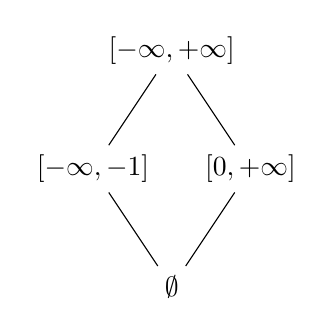
\begin{tikzpicture}
    \node (a)  at (0,0) {$[-\infty, +\infty]$};
    \node (b1) at (1,-1.5) {$[0,+\infty]$};
    \node (b2) at (-1,-1.5) {$[-\infty, -1]$};
    \node (c) at (0,-3) {$\emptyset$};
    \draw (a) to (b1);
    \draw (a) to (b2);
    \draw (b1) to (c);
    \draw (b2) to (c);
\end{tikzpicture}
    \caption{Hasse diagram of $C_\mathcal{I}(\uints)$}
    \label{fig:termination-example-cover-lattice}
\end{figure}

